\section{Experiment}
\label{sec:experiment}

\subsection{Dataset and Training Setup}
Following Meta CLIP pipeline, we collect image-text pairs sourced from the Internet that are publicly available.
After LID, there are about 44\% of alt-texts are in English, which are on par with the scale of English-only data from Meta CLIP~\citep{xu2024demystifying}. 
For generalizable recipe and findings, we base our training setup on OpenAI CLIP's ViT-L/14 and Meta CLIP ViT-H/14, except changes necessary for enabling worldwide capability, as described in Sec.~\ref{sec:scaling_recipe} and ablated in later subsections. The full details can be found in Table \ref{tbl:hp} and Appendix~\ref{sec:training_setup}.

\subsection{Evaluation}
\label{sec:main}

We first present the main ablations of Meta CLIP~2 on a wide range of English and multilingual zero-shot transfer benchmarks, along with other multilingual CLIP baselines for comparison (Sec.~\ref{sec:main_ablation}); then 
we conduct a comprehensive ablation study on the variants of metadata, curation and tokenizer (Sec.~\ref{sec:ablation_metadata_curation_tokenizer}).
Lastly, we evaluate the embedding quality of Meta CLIP~2 on downstream tasks for culture diversity (Sec.~\ref{sec:cultural}).
Additionally, we conduct analysis on embedding alignment and uniformity~\citep{wang2020hypersphere} in Sec.~\ref{appx:align_uni}.

\subsubsection{Main Ablation}
\label{sec:main_ablation}
We first ablate the effects of scaling seen training pairs and minimal viable model capacity that break the curse of multilinguality, 
with the following two groups of 6 training runs. Two trainings are in ViT-L/14 on worldwide curated data and its English portion, where global batch size and seen pairs are set to 2.3$\times$ and 1.0$\times$ compared to OpenAI CLIP and Meta CLIP setting (i.e., 1.0$\times$ has 12.8B seen pairs, or 400M for 32 epoches as in OpenAI CLIP). Four runs are on ViT-H/14 with different subsets of curated data to demonstrate the effects of English data helping multilingual performance and vice versa. We denote each run based on subsets trained with and corresponding seen pairs: 1) Worldwide (2.3$\times$) with the full-fledged worldwide curated data; 2) Worldwide (1.0$\times$) with 1) downsampled; 3) English (1.0$\times$) with English portion of 1); 4) Non-English (1.3$\times$) with the non-English portion.

We adopt the following two groups of zero-shot transfer benchmarks: 1) \textit{English-only} benchmarks on \textbf{ImageNet (IN val)}~\citep{russakovsky2015imagenet}, 
\textbf{SLIP 26 tasks (SLIP 26 avg.)}~\citep{mu2021slip},
and \textbf{DataComp 37 tasks (DC 37 avg.)}~\citep{gadre2023datacomp};
2) \textit{multilingual} benchmarks on \textbf{Babel-ImageNet (Babel-IN)}~\citep{geigle2024babel} (averaged zero-shot classification on IN with classes and prompts translated into 280 languages), 
\textbf{XM3600}~\citep{thapliyal2022crossmodal} (multilingual text-to-image, T→I, and image-to-text, I→T, retrieval with an averaged  recall@1 on 36 languages),
\textbf{CVQA}~\citep{mogrovejo2024cvqa} (multilingual multi-choice visual question answering with English and local averaged answer accuracy),
\textbf{Flickr30k-200}~\citep{visheratin2023nllb} (Flickr30k test set translated into 200 languages), 
\textbf{XTD-10}~\citep{aggarwal2020towards} (multilingual image-text retrieval on MSCOCO~\citep{chen2015microsoft} averaged Recall@1 over 7 languages), and \textbf{XTD-200}~\citep{visheratin2023nllb} (XTD10 translated into 200 languages). The main ablation is shown in Table~\ref{tab:main_results}. We observe that Meta CLIP~2 on ViT-H/14 with worldwide data and scaled seen pairs consistently outperforms its counterparts English (1.0$\times$) and Non-English (1.3$\times$), on both English and multilingual tasks, effectively breaking the
``curse of multilinguality''. The curse still exists in non-scaled seen pairs, Worldwide (1.0$\times$) or smaller ViT-L/14 model even with Worldwide (2.3$\times$)).

\begin{table}[h]
\centering
\scalebox{0.58}{
\begin{tabular}{l|c|c|l|c|c|c|c|c|c|c|c|c}
\hline
& & & & \multicolumn{3}{c|}{\textbf{English Benchmarks}} & \multicolumn{6}{c}{\textbf{Multilingual Benchmarks}} \\
\cline{5-13}
\textbf{Model}  & \makecell{\textbf{ViT}\\\textbf{Size (Res.)}} & \textbf{Data} & \makecell{\textbf{Seen}\\\textbf{Pairs}} & 
\makecell{\textbf{IN}\\\textbf{val}} & \makecell{\small{\textbf{SLIP 26}}\\\textbf{avg.}} & \makecell{\small{\textbf{DC 37}}\\\textbf{avg.}} & \makecell{\textbf{Babel}\\\textbf{-IN}} & 

\makecell{\textbf{XM3600}\\T$\rightarrow$I I$\rightarrow$T} & 

\makecell{\textbf{CVQA}\\EN LOC} & 

\makecell{\small{\textbf{Flicker30k}}\\\small{\textbf{-200}}\\T$\rightarrow$I I$\rightarrow$T} & 

\makecell{\textbf{XTD-10}\\T$\rightarrow$I I$\rightarrow$T} & 

\makecell{\textbf{XTD-200}\\T$\rightarrow$I I$\rightarrow$T} \\
\hline
\g{\small{XLM-CLIP}\citep{ilharco_gabriel_2021_5143773}} & \g{H/14(224)} & \g{\small LAION-5B} & \g{32B (2.5$\times$)} & \g{77.0} & \g{69.4} & \g{65.5} & \g{34.0} & \g{50.4 /} \g{60.5} & \g{56.1 /} \g{48.2} & \g{43.2 /} \g{46.2} & \g{87.1 /} \g{88.4} & \g{42.5 /} \g{45.2} \\

\g{mSigLIP\citep{zhai2023sigmoid}} & \g{B/16(256)} & \g{WebLI(12B)} & \g{40B (3.0$\times$)} & \g{75.1} & \g{63.8} & \g{60.8} & \g{40.2} & \g{44.5 /} \g{56.6} & \g{51.8 /} \g{45.7} & \g{34.0 /} \g{36.0} & \g{80.8 /} \g{84.0} & \g{37.8 /} \g{40.6} \\

\g{mSigLIP\citep{zhai2023sigmoid}} & \g{\small SO400M(256)} & \g{WebLI(12B)} & \g{40B (3.0$\times$)} & \g{80.6} & \g{69.1} & \g{65.5} & \g{46.4} & \g{50.0 /} \g{62.8} & \g{56.8 /} \g{49.8} & \g{39.9 /} \g{42.0} & \g{85.6 /} \g{88.8} & \g{42.5 /} \g{45.2} \\
\g{SigLIP~2\citep{tschannen2025siglip}} & \g{\small SO400M(256)} & \g{WebLI(12B)} & \g{40B (3.0$\times$)}  & \g{83.2} & \g{73.7} & \g{69.4} & \g{40.8} & \g{48.2 /} \g{59.7} & \g{58.5 /} \g{49.0} & \g{36.6 /} \g{40.3} & \g{86.1 /} \g{87.6} & \g{40.3 /} \g{44.5}\\
\hline
\multirow{2}{*}{Meta CLIP\citep{xu2024demystifying}} & L/14(224) & English(2.5B) & 13B (1.0$\times$) & 79.2 & 69.8 & 65.6 & - & - \quad - & - \quad - & - \quad - & - \quad - & - \quad - \\
 & H/14(224) & English(2.5B) & 13B (1.0$\times$) & 80.5 & 72.4 & 66.5 & - & - \quad - & - \quad - & \g{- \quad -} & - \quad - & - \quad - \\
\hline

\multirow{2}{*}{Meta CLIP~2} & \multirow{2}{*}{L/14(224)} & English & 13B (1.0$\times$) & 79.5 & 69.5 & 66.0 & - & - \quad - & - \quad - & - \quad - & - \quad - & - \quad -\\

& & Worldwide & 29B (2.3$\times$) & 78.8 & 67.2 & 63.5 & 44.2 & 45.3 / 58.2 & 59.2 / 55.1 & 41.9 / 45.8 & 82.8 / 85.0 & 41.9 / 44.8\\
\hline
\multirow{4}{*}{Meta CLIP~2} & \multirow{4}{*}{H/14(224)} & English & 13B (1.0$\times$) & 80.4 & 72.6 & 68.7 & - & - \quad - & - \quad - & - \quad - & - \quad - & - \quad -\\

&  & Non-Eng. & 17B (1.3$\times$)& 71.4 & 63.1 & 61.7 & 49.9 & 46.9 / 59.9 & 59.8 / 56.8 & 47.5 / 50.5 & 83.2 / 85.7 & 46.6 / 49.2\\

&  & Worldwide & 13B (1.0$\times$)& 79.5 & 71.1 & 67.2 & 47.1 & 49.6 / 62.6 & 59.9 / 56.0 & 49.1 / 52.1 & 85.2 / 87.1 & 47.0 / 49.7\\
\rowcolor{lightpurple}
\cellcolor{white} & \cellcolor{white} & Worldwide & 29B (2.3$\times$) & 81.3 & 74.5 & 69.6 & 50.2 & 51.5 / 64.3 & 61.5 / 57.4 & 50.9 / 53.2 & 86.1 / 87.5 & 48.9 / 51.0\\
\hline
\end{tabular}

}
\vspace{1.5mm}
\caption{Main ablation: Meta CLIP~2 breaks the curse of multilinguality when adopting ViT-H/14, with seen pairs scaled (2.3$\times$) proportional to the added non-English data. Meta CLIP~2 outperforms mSigLIP with fewer seen pairs (72\%), lower resolution (224px vs. 256px), and comparable architectures (H/14 vs. SO400M). 
We \g{grey out} baselines those are SoTA-aiming systems with confounding factors. Here, numbers of seen pairs are rounded to the nearest integer (e.g., 12.8B->13B).
}
\label{tab:main_results}
\end{table}

Although SoTA is non-goal for Meta CLIP~2, its full recipe
demonstrates strong performance
with fewer seen pairs (72\% of SigLIP series) and lower resolution (224px vs mSigLIP's 256). Meta CLIP~2 surpasses mSigLIP on IN, SLIP 26, and DC 37, and the recent SigLIP 2 on later two. More significantly, Meta CLIP~2 sets many SoTA multilingual benchmarks, e.g., Babel-IN (+3.8\%), XM3600 (+1.1\%/+1.5\%), CVQA (+3\%/+7.6\%), Flicker-30k-200 (+7.7\%/+7\%), and XTD-200 (+6.4\%/+5.8\%). SigLIP~2 prioritizes English (90\% of its training data in English), while it is worse than mSigLIP on multilingual tasks and Meta CLIP~2 on most English benchmarks except IN.

\begin{table}[h]
\centering
\small
\scalebox{0.88}{
\begin{tabular}{l|l|l|c|c|c c|c c}
\hline

\textbf{Ablation Steps} & \textbf{Metadata} & \textbf{Alt-texts} & \textbf{IN} & \textbf{Babel-IN} & \multicolumn{2}{c|}{\makecell{\textbf{XM3600}\\T$\rightarrow$I I$\rightarrow$T} } & \multicolumn{2}{c}{\makecell{\textbf{CVQA}\\EN LOCAL} }\\
\hline
1: English CLIP & English & English & \bf 67.5 & - & - & - & - & - \\
2: remove English filter & English & all, in 1 set & 66.9 & - & - & - & - & - \\

3: no language isolation & all, in 1 set & all, in 1 set & 62.1 & 31.2 & 37.8 & 49.7 & 49.8 & 45.8\\

4: language isolation with $t_\text{lang}=t_\text{en}$ & all, by lang. & all, by lang. & 61.1 & \bf 31.5 & 37.9 & 49.4 & 49.0 & 46.5\\

5: language specific $t_\text{lang}$ & all, by lang. & all, by lang. & 64.7 & \bf 31.5 & \bf 38.1 & \bf 50.0 & \bf 50.3 & \bf 46.6\\
\hline
\end{tabular}
}
\vspace{1.5mm}
\caption{Ablation study of metadata and alt-texts combination on ViT-B/32 using English 1.0$\times$ and Worldwide 1.0$\times$ with mT5 multilingual tokenizer. $t_\text{lang}$ is the count thresholds for each language and $t_\text{en}$ for English.}
\label{tbl:ablation_metadata_curation}
\end{table}
\vspace{-3.mm}

\subsubsection{Ablation on Metadata, Curation, and Tokenizer}
\label{sec:ablation_metadata_curation_tokenizer}
We further ablate the transition from metadata and curation focuses solely on English to their worldwide equivalents using the ViT-B/32 encoder for efficiency.
We evaluate zero-shot transfer on IN for English and Babel-IN, XM3600 and CVQA for multilingual. As in Table~\ref{tbl:ablation_metadata_curation}, starting from English-only CLIP, we first remove the English filter on alt-texts so that all alt-texts are curated by English metadata, resulting in 0.6\% drop on IN, indicating English isolation separating text or metadata by LID before matching is important. Then, we replace English metadata using all metadata merged without separation, yielding even worse English performance but start building up multilingual capability. Next, we isolate substring matching and curate alt-text language-by-language, with the same $t_\text{en}$ over all languages. This further lowers English performance since $t_\text{en}$ is too high for non-English and let head data dominate curation.
Lastly, we compute $t_\text{lang}$, to keep the same ratio of head-to-tail concepts for each language. This improves English and non-English performance, while curse of multilinguality remains unresolved in ViT-B/32 until the main ablation described above.

To minimize changes in model architecture, we only swap the English tokenizer for a multilingual one. Four popular tokenizers are studied on our zero-shot benchmarks. As shown in Table~\ref{tbl:tokenizer_ablation}, the XLM-V vocabulary yields the strongest performance in both the English and non-English world.

\begin{table}[h]
\centering
\scalebox{0.9}{
\begin{tabular}{l|c|c|c|c c|c c}
\hline

\textbf{Tokenizer} & \textbf{Vocab. Size} & \textbf{IN val} & \textbf{Babel-IN avg.} & \multicolumn{2}{c|}{\makecell{\textbf{XM3600}\\T$\rightarrow$I I$\rightarrow$T} } & \multicolumn{2}{c}{\makecell{\textbf{CVQA}\\EN LOCAL} } \\
\hline
mT5 (mSigLIP) \citep{xue2020mt5} & 250k & \bf 64.7 & 31.5 & 38.1 & 50.0 & 50.3 & 46.6 \\
Gemma (SigLIP~2) \citep{team2024gemma} & 256k & 63.7 & 26.1 & 36.1 & 47.8 & 48.3 & 44.0 \\
XLM-Roberta \citep{conneau2019unsupervised} & 250k & 64.0 & 31.1 & 38.0 & 49.8 & 49.8 & 46.1\\
XLM-V \citep{liang2023xlm} & 900k & \textbf{64.7} & \textbf{32.7} & \textbf{40.0} & \textbf{51.4} & \textbf{50.4} & \textbf{47.4} \\
\hline
\end{tabular}
}
\vspace{1.5mm}
\caption{Ablation study of various multilingual tokenizers with ViT-B/32 and Worldwide 1.0$\times$.}
\label{tbl:tokenizer_ablation}
\end{table}
\vspace{-3.mm}

\subsubsection{Cultural Diversity}
\label{sec:cultural}

Following protocols in \cite{pouget2024no} and \cite{wang2025scaling}, we perform zero-shot classification and few-shot geo-localization on a range of geographically diverse benchmarks. Specifically, we include zero-shot classification with Dollar Street~\citep{gaviria2022dollar}, GeoDE~\citep{ramaswamy2023geode}, and GLDv2~\citep{weyand2020google} in Table~\ref{tbl:culture}, and few-shot geo-localization~\citep{pouget2024no} on Dollar Street, GeoDE and XM3600 
in Fig.~\ref{fig:culture}. We find that only changing the training data distribution, from 13B \emph{English} to 13B \emph{worldwide} pairs, yields significantly better performance, and scaling to 29B \emph{worldwide} pairs improves further,
except for the on-par, probably saturated performance in GeoDE. Fig. \ref{fig:culture} shows similar trend for evaluating on few-shot geo-localization.
\vspace{-2.mm}

\begin{table}[h]
\centering
\scalebox{0.87}{
\begin{tabular}{l|l|l|c c c c}
\hline
\textbf{Model} & \textbf{Data} & \textbf{Seen Pairs} & \multicolumn{2}{c}{\makecell{\textbf{Dollar Street} \\ Top-1\quad Top-5}} & \textbf{GLDv2} & \textbf{GeoDE} \\
\hline
\g{mSigLIP~\citep{zhai2023sigmoid}} & \g{WebLI(12B)~\citep{chen2023pali}} & \g{40B (3.0$\times$)} & \g{36.0} & \g{62.5} & \g{45.3} & \g{94.5} \\
\g{SigLIP~2~\citep{tschannen2025siglip}} & \g{WebLI(12B)~\citep{chen2023pali}} & \g{40B (3.0$\times$)} & \g{36.7} & \g{61.9} & \g{48.5} & \g{95.2} \\
\hline
\multirow{4}{*}{Meta CLIP~2} & English & 13B (1.0$\times$) & 37.2 & 63.3 & 52.8 & 93.4 \\
& Non-English & 17B (1.3$\times$) & 35.7 & 61.3 & 68.6 & 91.7 \\
& Worldwide & 13B (1.0$\times$) & 37.2 & 63.7 & 65.8 & 94.3 \\
\rowcolor{lightpurple}
\cellcolor{white} & Worldwide & 29B (2.3$\times$) & 37.9 & 64.0 & 69.0 & 93.4 \\
\hline
\end{tabular}
}
\caption{Zero-shot classification accuracy on cultural diversity benchmarks. Meta CLIP~2 models are in ViT-H/14 and mSigLIP/SigLIP~2 are in ViT-SO400M. mSigLIP/SigLIP~2 are SoTA-aiming systems with many factors changed and thus greyed out.}

\label{tbl:culture}
\vspace{-3.5mm}
\end{table}

\begin{figure}[h]
    \centering
    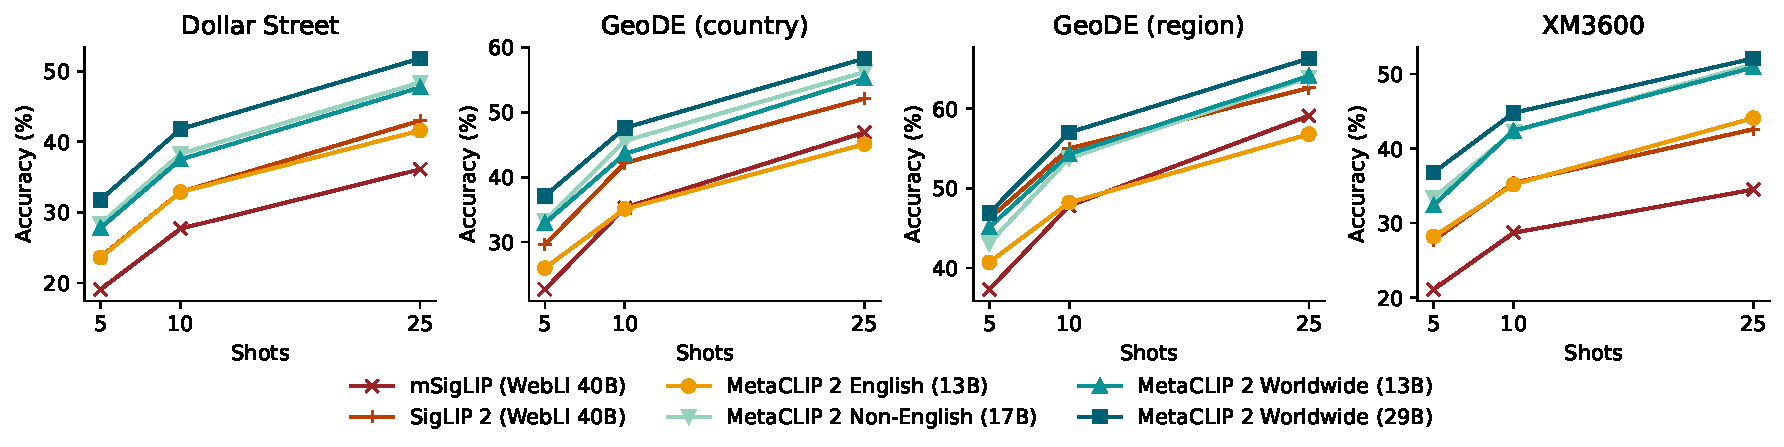
\includegraphics[width=\textwidth]{imgs/geo_results.pdf}
    \caption{Few-shot geo-localization accuracy on cultural diversity benchmarks.
    }
    \label{fig:culture}
\end{figure}

\subsubsection{Alignment and Uniformity}
\label{appx:align_uni}
Following~\citep{wang2020hypersphere}, we further measure the embeddings quality across different CLIP models.
To avoid various unknown biases from different benchmarks, we use 5k holdout image-text pairs not used in our training and report alignment and uniformity scores, where alignment measures the relevance of an image and a text and uniformity measures how images distributed in vision encoder's embedding space. Note that we have no control on whether these 5k pairs are leaked in other baselines.
From Fig. \ref{fig:alignment_uniformity}, we can see that Meta CLIP~2 exhibits good scores in both alignment and uniformity (lower is better), whereas mSigLIP or SigLIP~2 may have non-trivial bias on our collected holdout data.

\begin{figure}[h]
    \centering
    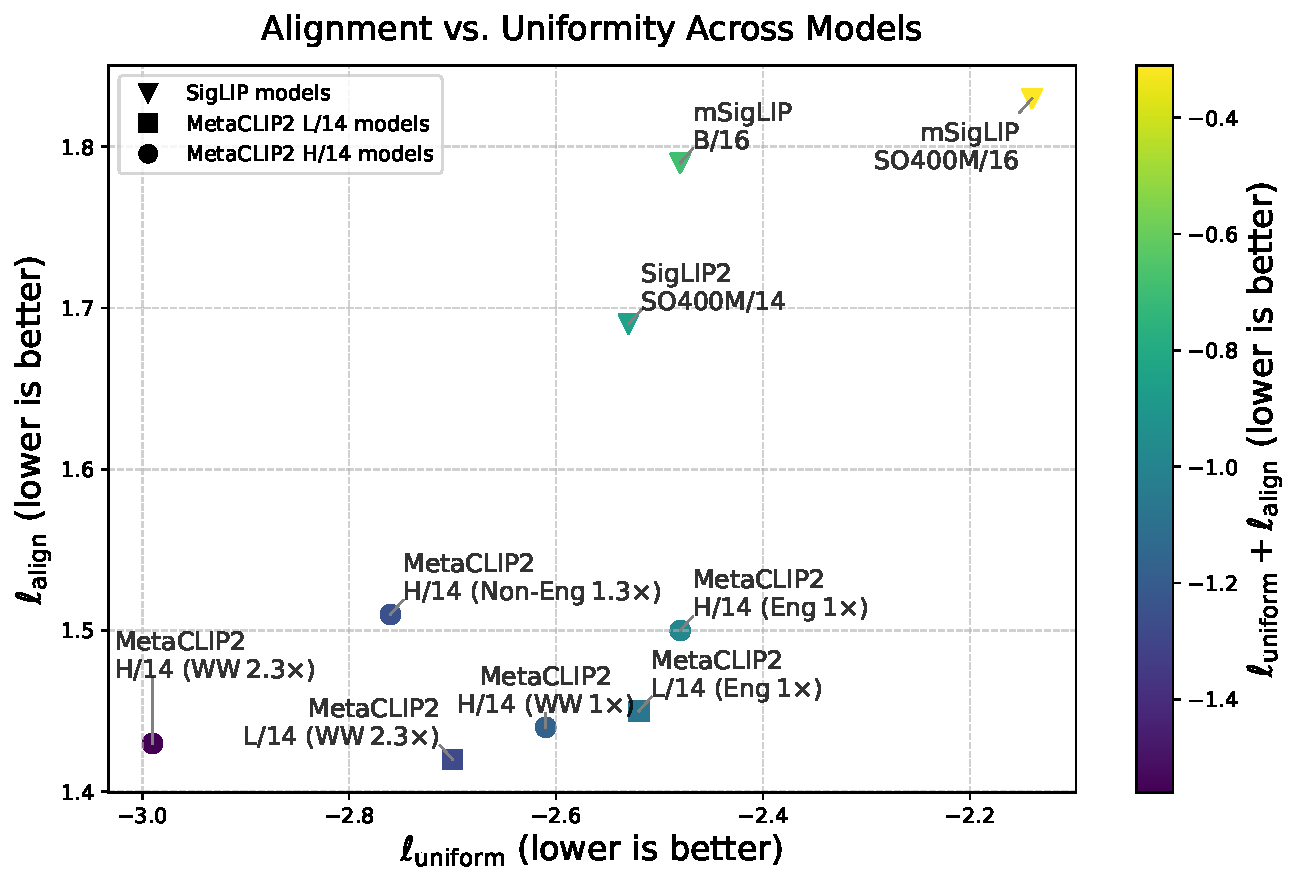
\includegraphics[width=0.8\textwidth]{imgs/align_uni.pdf}
    \caption{Alignment and uniformity scores~\citep{wang2020hypersphere} calculated on our collected 5k holdout data, WW indicates worldwide data.
    }
    \label{fig:alignment_uniformity}
\end{figure}
